\documentclass[9pt,aspectratio=169]{beamer}
\usepackage[T1]{fontenc}
\usepackage[utf8]{inputenc}
\usepackage{lmodern}
\usepackage{graphicx}
\usepackage{booktabs}
\usepackage{array}
\usepackage{xcolor}
\usepackage{ragged2e}

\definecolor{navy}{HTML}{1F3A5F}
\definecolor{teal}{HTML}{2A9D8F}
\definecolor{orange}{HTML}{E76F51}
\definecolor{gold}{HTML}{E9C46A}
\definecolor{grey}{HTML}{8D99AE}

\usetheme{default}
\usecolortheme{default}
\setbeamercolor{palette primary}{bg=navy,fg=white}
\setbeamercolor{palette secondary}{bg=navy,fg=white}
\setbeamercolor{palette tertiary}{bg=navy,fg=white}
\setbeamercolor{title}{fg=navy}
\setbeamercolor{frametitle}{bg=navy,fg=white}
\setbeamercolor{structure}{fg=navy}
\setbeamercolor{block title}{bg=teal,fg=white}
\setbeamercolor{block body}{bg=teal!8}
\setbeamertemplate{navigation symbols}{}
\setbeamertemplate{footline}[frame number]
\setbeamerfont{frametitle}{series=\bfseries}
\setbeamertemplate{itemize items}[circle]
\setbeamertemplate{itemize subitem}[triangle]

\newcommand{\good}{\textcolor{teal}{\textbf{Addressed}}}
\newcommand{\feedbacktag}[1]{{\small\textcolor{grey}{\textbf{Feedback:}~#1}}}

\title{\textbf{Capitolis Counterparty Credit Risk Engine}}
\subtitle{Methods, Results, and How Every Round of Feedback Was Incorporated}
\author{Berkeley MFE Industry Project}
\date{\today}

\begin{document}

\begin{frame}
  \titlepage
\end{frame}

% ============================================================ PART 1: CORE METHODS (crisp)
\begin{frame}{The book, and where every input comes from}
  \begin{columns}[T]
    \begin{column}{0.55\textwidth}
      \textbf{The book: 16 trades, 3 counterparties}
      \begin{itemize}
        \item 8 equity total-return swaps
        \item 4 bond forwards, 4 bond total-return swaps
        \item 37 equities (US + Tokyo) + USDJPY
      \end{itemize}
      \vspace{6pt}
      \textbf{Every input is real, sourced data}
      \begin{itemize}
        \item Equities/dividends: Yahoo Finance
        \item USD curve: bootstrapped from real Databento SOFR futures
        \item Treasury yields: FRED
        \item Long end + vol cube: licensed Bloomberg data, spliced in and cross-checked against public sources
      \end{itemize}
    \end{column}
    \begin{column}{0.45\textwidth}
      \textbf{Exposure definition (the brief):}
      \[ \max\big(V(t{+}10\text{bd}) - V(t{-}1\text{bd}),\,0\big) \]
      \begin{itemize}
        \item Signed prior-day variation margin
        \item No initial margin, no threshold
        \item Netted per counterparty only
      \end{itemize}
      \vspace{8pt}
      \textbf{Secondary view:} uncollateralized level exposure $\max(V(t),0)$ -- a no-margin upper bound
    \end{column}
  \end{columns}
\end{frame}

\begin{frame}{The simulation engine, in four bullets}
  \begin{itemize}
    \item \textbf{Equities \& FX:} correlated geometric Brownian motion, real 39$\times$39 correlation matrix (3-year realised)
    \item \textbf{USD rates:} one-factor Hull-White; mean reversion fitted to the swaption market, volatility fitted to realised \emph{long-end} Treasury vol (0.96\%, $a$=0.0167)
    \item \textbf{JPY rates:} a second, independent Hull-White factor from the real JPY OIS curve -- so JPY names and USDJPY move with real JPY rate risk, not a constant assumption
    \item \textbf{Sampling:} Latin Hypercube throughout; every sensitivity reuses the identical random draws in the base and shocked run (common random numbers)
  \end{itemize}
  \vspace{10pt}
  \begin{columns}[T]
    \begin{column}{0.5\textwidth}
      \centering \small
      \begin{tabular}{lr}
        \toprule
        Scenarios (standard) & 5,000 \\
        Scenarios (sign-off) & 10,000 \\
        Reporting horizon & 1 year \\
        \bottomrule
      \end{tabular}
    \end{column}
    \begin{column}{0.5\textwidth}
      \centering \small
      \begin{tabular}{lr}
        \toprule
        Automated tests & 168 \\
        Report length & 77 pages \\
        \bottomrule
      \end{tabular}
    \end{column}
  \end{columns}
\end{frame}

\begin{frame}{Headline results (5,000 scenarios, close-out exposure)}
  \begin{columns}[T]
    \begin{column}{0.42\textwidth}
      \small
      \begin{tabular}{lrr}
        \toprule
        & \textbf{MPE99} & \textbf{Peak EE} \\
        \midrule
        CPTY\_A & \$25.9M & \$4.7M \\
        CPTY\_B & \$9.6M & \$1.8M \\
        CPTY\_C & \$29.6M & \$5.2M \\
        \midrule
        \textbf{Portfolio} & \textbf{\$51.0M} & \textbf{\$11.6M} \\
        \bottomrule
      \end{tabular}
      \vspace{8pt}
      \begin{itemize}
        \item Portfolio MPE99 = 78\% of the sum (\$65.1M): no netting across counterparties, but exposures peak in the same weeks and are positively correlated
        \item CVA \$11.7k close-out / \$247k level
        \item SA-CVA capital \$0.10M / \$2.23M
        \item SA-CCR EAD \$260M
      \end{itemize}
    \end{column}
    \begin{column}{0.58\textwidth}
      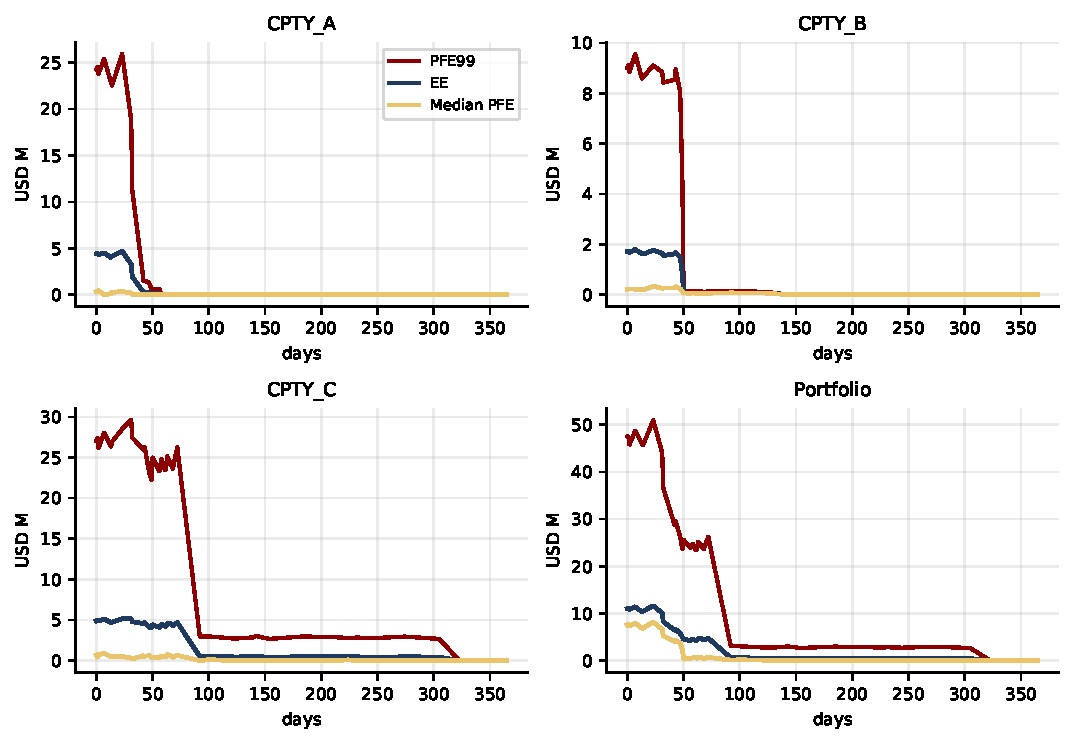
\includegraphics[width=\linewidth]{figures/fig25.pdf}
    \end{column}
  \end{columns}
\end{frame}

\begin{frame}{Close-out vs.\ level exposure: two brackets on the truth}
  \begin{columns}[T]
    \begin{column}{0.48\textwidth}
      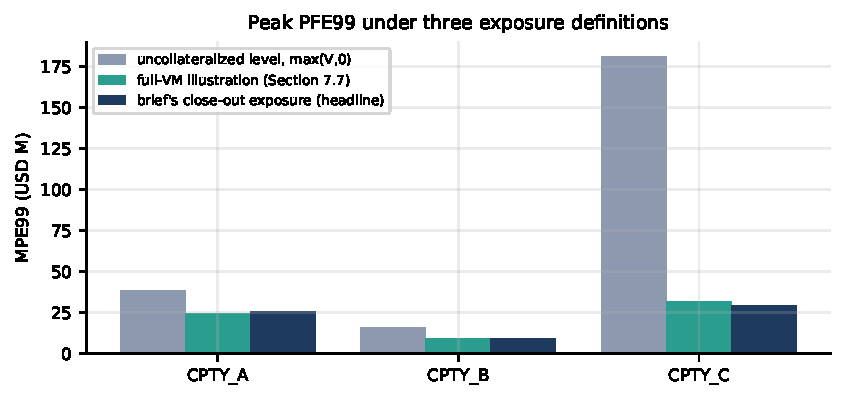
\includegraphics[width=\linewidth]{figures/fig26.pdf}
    \end{column}
    \begin{column}{0.52\textwidth}
      \small
      \begin{itemize}
        \item \textbf{Close-out} (the brief, primary): only the 10-day move from an already-margined start. Portfolio MPE99 \textbf{\$51.0M}.
        \item \textbf{Level} (secondary): whole mark-to-market at risk, no margin. Portfolio MPE \textbf{\$201.9M} -- driven by CPTY\_C's bond forward.
        \item The real answer sits between the two, depending on the actual CSA's threshold, MTA, and initial margin -- none of which were supplied.
      \end{itemize}
    \end{column}
  \end{columns}
\end{frame}

\begin{frame}{Stress testing methodology}
  \begin{columns}[T]
    \begin{column}{0.5\textwidth}
      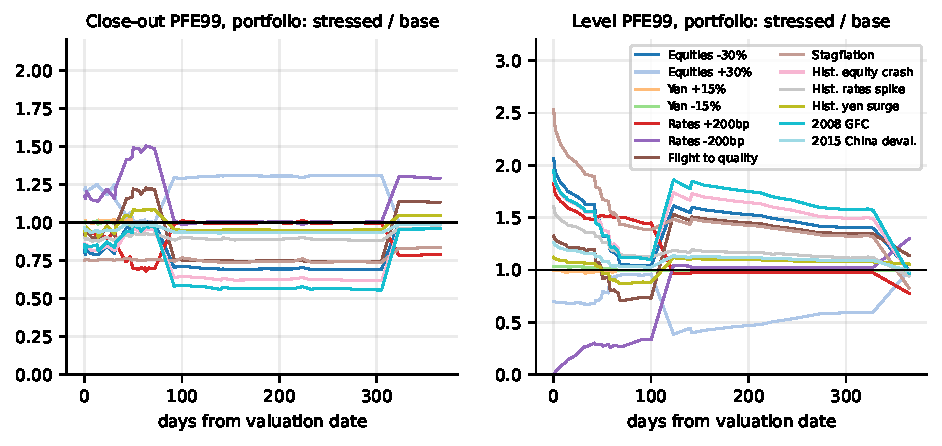
\includegraphics[width=\linewidth]{figures/fig33.pdf}
    \end{column}
    \begin{column}{0.5\textwidth}
      \small
      \textbf{13 fixed scenarios}, same random draws as the base case:
      \begin{itemize}
        \item 8 hypothetical: equities $\pm$30\%, yen $\pm$15\%, rates $\pm$200bp, flight-to-quality, stagflation
        \item 5 historical replays, chosen by rule (worst 10-day window), not by hand
      \end{itemize}
      Read at every reporting date, every trade, every counterparty -- not a one-paragraph narrative.
    \end{column}
  \end{columns}
\end{frame}

\begin{frame}{Sensitivities (Greeks): method}
  \begin{itemize}
    \item Bump-and-reprice with \textbf{common random numbers}: same draws in base and bumped run, so the difference is signal, not noise
    \item Equity/FX bumps: rescale the simulated GBM paths exactly -- \textbf{no resimulation}
    \item Rate/vol bumps: require a genuine resimulation
    \item Pathwise (closed-form) estimator implemented for equity/FX as a fast cross-check
  \end{itemize}
  \vspace{6pt}
  \centering
  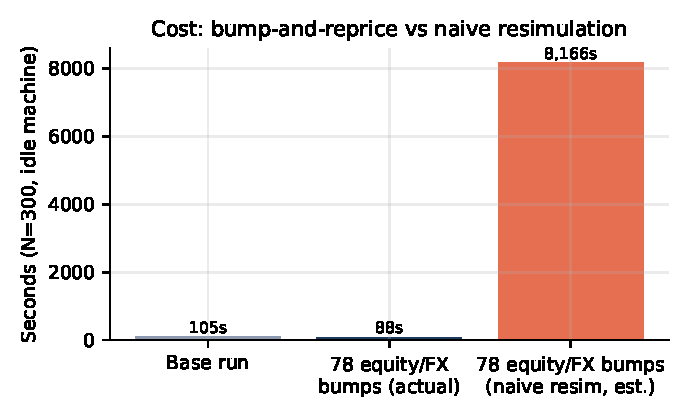
\includegraphics[width=0.62\linewidth]{figures/fig_greeks_cost.pdf}
\end{frame}

\begin{frame}{CVA, DVA, FVA: the credit and funding adjustments}
  \begin{columns}[T]
    \begin{column}{0.48\textwidth}
      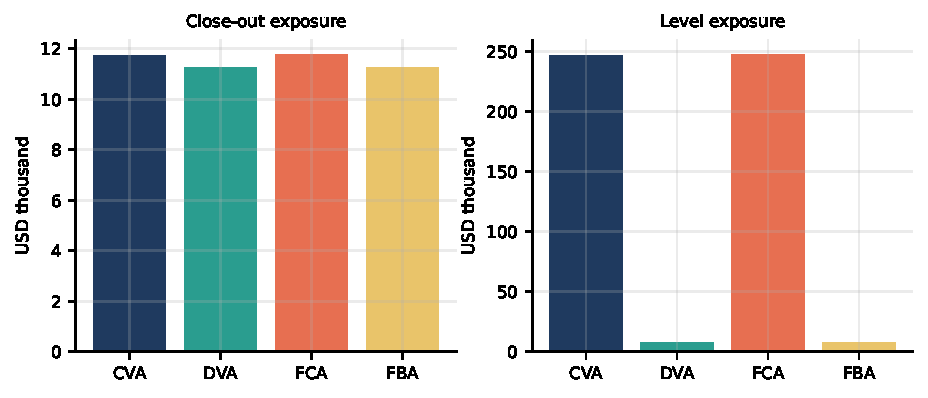
\includegraphics[width=\linewidth]{figures/fig38.pdf}
    \end{column}
    \begin{column}{0.52\textwidth}
      \small
      \begin{itemize}
        \item \textbf{CVA:} expected loss from counterparty default, credit-triangle default probabilities from BBB bond-index spread proxies
        \item \textbf{DVA:} mirror image -- our own default risk on what we owe them
        \item \textbf{FVA:} funding cost of positive exposure less funding benefit of negative exposure
        \item \textbf{SA-CVA:} Basel standardised-approach capital from CVA's own market-risk sensitivities
      \end{itemize}
    \end{column}
  \end{columns}
\end{frame}

% ============================================================ PART 2: FEEDBACK TRACKER (summary)
\begin{frame}{Feedback tracker: everything raised, everything addressed}
  \small
  \textbf{Earlier meeting} (5 items) \hfill \textbf{This meeting} (6 items)
  \vspace{4pt}
  \begin{columns}[T]
    \begin{column}{0.48\textwidth}
      \begin{enumerate}
        \item Robust stress testing \good
        \item Sensitivities: method, cost, faster alternative \good
        \item PCA explainability and speed \good
        \item Final results explanation \good
        \item CVA walkthrough and set-up \good
      \end{enumerate}
    \end{column}
    \begin{column}{0.48\textwidth}
      \begin{enumerate}
        \item[6.] 2008 and more testing periods \good
        \item[7.] LHS to calculate sensitivities \good
        \item[8.] KVA addition \good
        \item[9.] CVA is for sensitivities, not the number \good
        \item[10.] DV01 via a Jacobian \good
        \item[11.] Excel parametric vol-bump test \good
      \end{enumerate}
    \end{column}
  \end{columns}
  \vspace{10pt}
  \centering \small \textcolor{grey}{The next 11 slides take each item in turn: what was asked, what we did, the results, and the conclusion.}
\end{frame}

% ============================================================ earlier feedback, one slide each
\begin{frame}{1. Robust stress testing}
  \feedbacktag{make it a robust, structured test, not a paragraph -- data, inputs, sensitivity along the path, all products}
  \vspace{6pt}
  \begin{columns}[T]
    \begin{column}{0.5\textwidth}
      \textbf{What we did}
      \begin{itemize}
        \item 13 scenarios (8 round-number, 5 historical), each a full re-run of the Monte Carlo from the shocked state, same random draws as base
        \item Results read at every reporting date, every trade, every counterparty
        \item A per-trade heat map shows exactly which products move under which shocks
      \end{itemize}
    \end{column}
    \begin{column}{0.5\textwidth}
      \textbf{Result / finding}
      \begin{itemize}
        \item Close-out MPE99 moves at most $-24\%$ to $+23\%$; level MPE99 moves up to $+89\%$ -- margin is why
        \item Equity swaps respond only to equity/FX shocks; bond forwards/TRS respond only to rate shocks -- confirms trade structure, not a coincidence
      \end{itemize}
      \vspace{6pt}
      \textbf{Conclusion:} stress sensitivity is now quantified, dated, and attributable to a specific shock -- not a qualitative claim.
    \end{column}
  \end{columns}
\end{frame}

\begin{frame}{2. Sensitivities: method, cost, faster alternative}
  \feedbacktag{explain how Greeks are generated, what they cost, and whether something faster exists}
  \begin{columns}[T]
    \begin{column}{0.5\textwidth}
      \textbf{Method}
      \begin{itemize}
        \item Bump-and-reprice, common random numbers (CRN)
        \item CRN cuts estimator noise from \$245k to \$1k -- 282x
      \end{itemize}
      \textbf{Cost (N=300, 8 cores)}
      \begin{itemize}
        \item Base run: 105s
        \item 78 equity/FX bumps: 88s (vs.\ $\sim$8,200s naive -- 93x cheaper)
        \item Rate/vol bumps: still need resimulation, $\sim$109s each
      \end{itemize}
    \end{column}
    \begin{column}{0.5\textwidth}
      \textbf{Faster alternative}
      \begin{itemize}
        \item Pathwise (closed-form) delta for equity/FX: 0.2--0.4s vs.\ $\sim$260s for bump-and-reprice
        \item Validated against bump-and-reprice: median 0.02\%, worst 0.4\% difference
      \end{itemize}
      \vspace{6pt}
      \textbf{Conclusion:} common random numbers is what actually controls Greeks noise; pathwise is a validated, production-ready shortcut for linear (equity/FX) risk only.
    \end{column}
  \end{columns}
\end{frame}

\begin{frame}{3. PCA explainability and speed}
  \feedbacktag{improve the explainability of the PCA factor model, and quantify the speed it adds}
  \begin{columns}[T]
    \begin{column}{0.5\textwidth}
      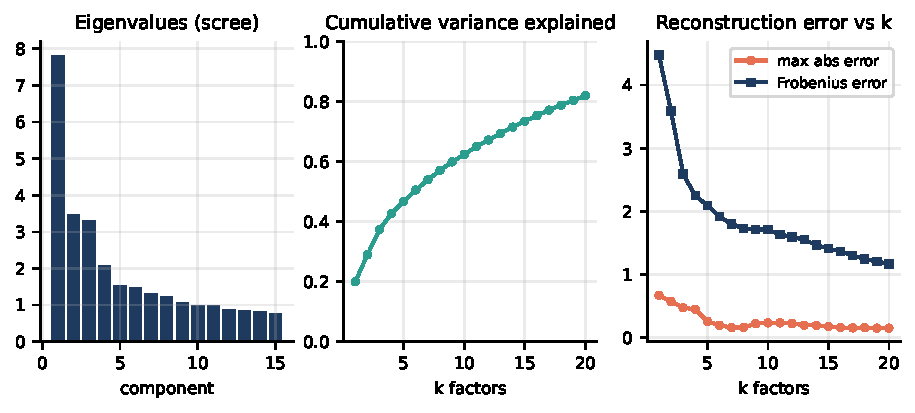
\includegraphics[width=\linewidth]{figures/fig14.pdf}
    \end{column}
    \begin{column}{0.5\textwidth}
      \textbf{Explainability}
      \begin{itemize}
        \item Factor 1 (20\% of variance): a broad market factor
        \item Factor 2 (8.9\%): Japan vs.\ US
        \item 5 factors explain 47\%; 10 factors explain 62\%
      \end{itemize}
      \textbf{Speed: measured honestly, found to be none}
      \begin{itemize}
        \item Full matrix: 1.91s per correlated-shock step
        \item 5-factor PCA: 2.08s; 10-factor: 2.29s -- \emph{slower}, not faster
      \end{itemize}
      \vspace{4pt}
      \textbf{Conclusion:} kept the full matrix as default; PCA stays as an explainable robustness check, not a speed optimisation.
    \end{column}
  \end{columns}
\end{frame}

\begin{frame}{4. Final results: what drives each counterparty}
  \feedbacktag{confirm A=equity, C=rates, bonds vs.\ equities inversely, and why the portfolio is so close to additive}
  \begin{columns}[T]
    \begin{column}{0.55\textwidth}
      \small
      \begin{tabular}{lrr}
        \toprule
        & \textbf{Equity $\Delta$/+1\%} & \textbf{DV01/+1bp} \\
        \midrule
        CPTY\_A & -\$2.25M & \$31k \\
        CPTY\_B & -\$0.96M & -\$4k \\
        CPTY\_C & -\$1.24M & \textbf{\$594k} \\
        \bottomrule
      \end{tabular}

      \vspace{8pt}
      \small
      Rank correlation of exposures: A--B 0.34, A--C 0.33, B--C 0.12
    \end{column}
    \begin{column}{0.45\textwidth}
      \small
      \begin{itemize}
        \item A is the most equity-driven; C is the rate netting set (one \$500M short forward on a 2049 Treasury) -- but C also carries meaningful equity delta
        \item Yield-equity correlation in our data is $\approx$0.00 -- the ``inverse'' relationship is regime-dependent, not fixed
        \item Portfolio MPE99 (\$51.0M) is close to A+C (\$54.4M): nothing nets \emph{across} counterparties by construction, and the three books peak in the same weeks
      \end{itemize}
    \end{column}
  \end{columns}
\end{frame}

\begin{frame}{5. CVA walkthrough and set-up for next session}
  \feedbacktag{walk through the CVA calculation in full, and set up the open questions for next time}
  \begin{columns}[T]
    \begin{column}{0.5\textwidth}
      \textbf{Steps (CPTY\_C example)}
      \begin{enumerate}
        \item Exposure profile from the simulation, discounted along each path
        \item Default probability from a credit spread (BBB proxy: 59bp at 1y, 91bp at 5y) via the credit triangle
        \item LGD 60\%; multiply and sum
      \end{enumerate}
    \end{column}
    \begin{column}{0.5\textwidth}
      \textbf{Results}
      \begin{itemize}
        \item CPTY\_C close-out CVA \$8k; total \$12k
        \item Rating sensitivity: AA \$7k, A \$8k, BBB \$12k, BB \$18k
      \end{itemize}
      \vspace{6pt}
      \textbf{Set-up for next time:} exposure convention, real ratings/CDS, own credit/funding spread, wrong-way risk, capital approach, margin terms -- six explicit open questions carried to today's deck.
    \end{column}
  \end{columns}
\end{frame}

% ============================================================ this meeting's feedback, one slide each
\begin{frame}{6. Add 2008, and more testing periods}
  \feedbacktag{add maybe 2008, add more testing periods}
  \begin{columns}[T]
    \begin{column}{0.5\textwidth}
      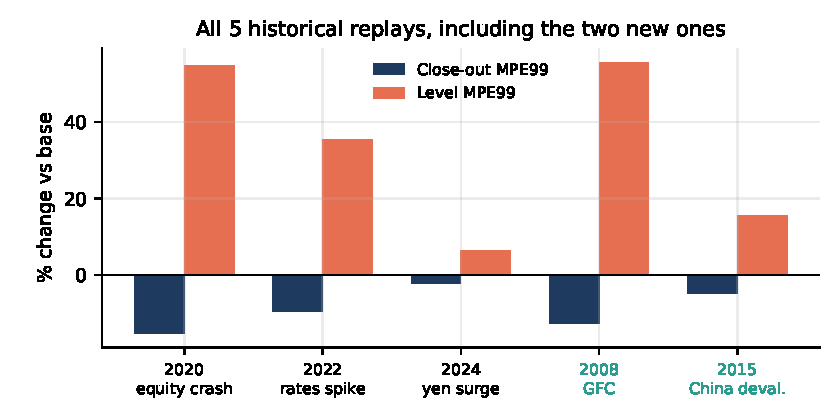
\includegraphics[width=\linewidth]{figures/fig_hist_scenarios.pdf}
    \end{column}
    \begin{column}{0.5\textwidth}
      \small
      \textbf{Method:} extended the public price history back to 2007 (28 of 37 names covered) and found the worst 10-day equity window inside two named crises, using the same objective rule as the existing replays.
      \begin{itemize}
        \item \textbf{2008 GFC:} Sep 29 -- Oct 10, 2008; $-23\%$ median / $-44\%$ worst single-name return
        \item \textbf{2015 China deval.:} Aug 2015, $-6.8\%$ median
      \end{itemize}
      \vspace{4pt}
      \textbf{Result:} 2008 moves close-out MPE99 by $-13\%$, level by $+56\%$ -- inside the range the existing scenarios already covered.
      \vspace{4pt}
      \textbf{Conclusion:} leaving out 2008 was not quietly understating the tail.
    \end{column}
  \end{columns}
\end{frame}

\begin{frame}{7. Use Latin Hypercube to calculate a sensitivity}
  \feedbacktag{is there a way to do the shock as part of this, like calculate sensitivities using this}
  \begin{columns}[T]
    \begin{column}{0.55\textwidth}
      \textbf{Method}
      \begin{itemize}
        \item In one-factor Hull-White, $r(t) = x(t) + \alpha(t)$
        \item $x(t)$: the simulated stochastic factor -- depends only on the random draws, $a$, $\sigma$
        \item $\alpha(t)$: purely deterministic, depends only on the curve
        \item A curve bump (fixed $a,\sigma$) leaves $x(t)$ \textbf{identical} to the base run
      \end{itemize}
    \end{column}
    \begin{column}{0.45\textwidth}
      \textbf{Result}
      \begin{itemize}
        \item The whole bump effect is one closed-form number per date, added to the base run's own paths
        \item \textbf{No resimulation. No new random draws.}
        \item Validated against a true independent resimulation: agreement to $\mathbf{10^{-15}}$ relative precision
      \end{itemize}
      \vspace{6pt}
      \textbf{Conclusion:} yes -- exactly, not approximately, for any curve-only bump under the one-factor model.
    \end{column}
  \end{columns}
\end{frame}

\begin{frame}{8. KVA addition}
  \feedbacktag{KVA addition, CVA, FVA, KVA}
  \begin{columns}[T]
    \begin{column}{0.48\textwidth}
      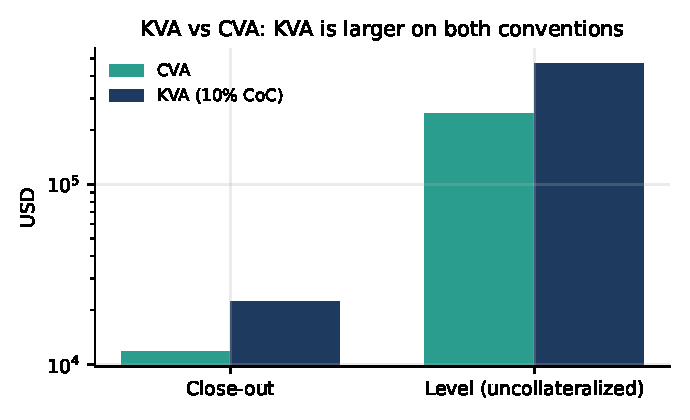
\includegraphics[width=\linewidth]{figures/fig_kva_compare.pdf}
    \end{column}
    \begin{column}{0.52\textwidth}
      \small
      \textbf{Method:} added KVA as a fourth, explicitly illustrative xVA term:
      \[ K(t) = 8\%\times\text{RW}\times\alpha\times\text{EPE}(t) \]
      discounted and integrated like CVA/DVA/FVA, scaled by an assumed cost of capital (8/10/12\% swept -- none given).

      \vspace{4pt}
      \textbf{Result at 10\% CoC:}
      \begin{itemize}
        \item KVA \$22.4k (close-out) vs.\ CVA \$11.7k
        \item KVA \$470k (level) vs.\ CVA \$247k
      \end{itemize}
      \textbf{Conclusion:} KVA exceeds CVA because it scales the whole EPE profile by a fixed ratio, not a small IG default probability -- explicitly illustrative, pending a real capital methodology.
    \end{column}
  \end{columns}
\end{frame}

\begin{frame}{9. CVA is mostly for understanding sensitivities}
  \feedbacktag{CVA is done mostly to understand Greeks / sensitivities calculations}
  \begin{columns}[T]
    \begin{column}{0.5\textwidth}
      \textbf{What this means in practice}
      \begin{itemize}
        \item The headline CVA number is small and not the point
        \item What a credit/XVA desk actually manages day to day is the \emph{sensitivity} of CVA to market and credit inputs
      \end{itemize}
    \end{column}
    \begin{column}{0.5\textwidth}
      \textbf{What we deliver as a result}
      \begin{itemize}
        \item CVA01: sensitivity to a 1bp move in the counterparty spread
        \item Full rating table: AAA \$5.0k $\to$ B \$32.8k
        \item SA-CVA weighted sensitivities by risk class (rates, FX, equity, credit spread)
      \end{itemize}
      \vspace{6pt}
      \textbf{Conclusion:} the report now states this framing explicitly, and the sensitivity chain is the deliverable, not the point estimate.
    \end{column}
  \end{columns}
\end{frame}

\begin{frame}{10. DV01 via a Jacobian: bump the curve, not just the zero rate}
  \feedbacktag{DV01 rates -- use Jacobian, bumping the curve (not just the zero rate?)}
  \begin{columns}[T]
    \begin{column}{0.5\textwidth}
      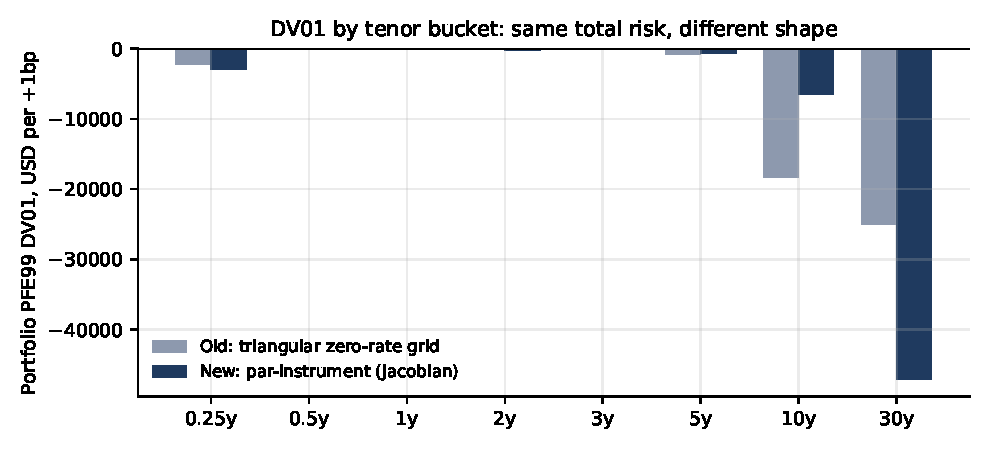
\includegraphics[width=\linewidth]{figures/fig_dv01_compare.pdf}
    \end{column}
    \begin{column}{0.5\textwidth}
      \small
      \textbf{Old method:} bump the \emph{fitted} zero curve at 8 hand-picked tenors, triangular in between.

      \textbf{New method:} bump the curve's own $\sim$45 native construction pillars (SOFR futures + Bloomberg long end), grouped into the same 8 buckets -- the genuine par-instrument sensitivity.

      \vspace{4pt}
      \textbf{Result:} the 30y bucket carries \textbf{82\%} of portfolio DV01 (new) vs.\ \textbf{54\%} (old) -- the old grid smeared the 20--50y risk (where the 2049 bond forward lives) into the 10y bucket. Bucket sums match the parallel bump to within 0.1\% either way.
    \end{column}
  \end{columns}
\end{frame}

\begin{frame}{11. Parametric test in Excel: bump equity vol}
  \feedbacktag{parametric testing using Excel of bumping vol of equities and showing}
  \small
  \begin{columns}[T]
    \begin{column}{0.5\textwidth}
      \textbf{Method}
      \begin{itemize}
        \item Bump one USD equity's vol $\pm$1\%
        \item Compute a simple ATM position's expected exposure $E[\max(S_T-S_0,0)]$ two ways: closed-form Black formula (live Excel formula), and Monte Carlo
      \end{itemize}
    \end{column}
    \begin{column}{0.5\textwidth}
      \textbf{Results}
      \begin{itemize}
        \item Level match: within $\sim$3\%
        \item Vega match: within $\sim$7\%
        \item (Realised vol formulas match calibration to 0.1\%; simulated vol matches analytic to 1--2\%)
      \end{itemize}
    \end{column}
  \end{columns}
  \vspace{6pt}
  \textbf{Conclusion:} every number in the workbook is a live spreadsheet formula on public data -- anyone can reproduce the engine's key numbers with a hand calculator.
\end{frame}

% ============================================================ next steps
\begin{frame}{Open questions to resolve before the next working session}
  \begin{itemize}
    \item Which exposure convention prices CVA in production: close-out, or level -- and what does the real CSA specify (threshold, MTA, IM)?
    \item Can real credit ratings or CDS-implied spreads be obtained for CPTY\_A/B/C (the BBB proxy currently drives every credit number)?
    \item Capitolis' own credit and funding spread for DVA/FVA (currently hypothetical and symmetric)?
    \item Should wrong-way risk be modelled (exposure/default independence is currently assumed)?
    \item What real capital methodology and cost of capital should be used for KVA (currently an assumed 8/10/12\% grid)?
    \item Adopt the two-factor G2++ rate model as production default? (Compared: changes portfolio MPE99 by only $-3\%$.)
  \end{itemize}
\end{frame}

\begin{frame}
  \centering
  \vspace{2cm}
  {\Huge \textcolor{navy}{\textbf{Thank you}}}\\[8pt]
  {\large Questions and discussion}
\end{frame}

\end{document}
